\documentclass[tikz,border=8pt]{standalone}
% Shared styles for the Hands-On 4 diagrams. Colours match the Hands-On 1 diagrams.
\usepackage{amsmath,amssymb}
\usetikzlibrary{positioning,calc,arrows.meta,decorations.pathreplacing,shapes.geometric}
\definecolor{tensorblue}{HTML}{3274B5}
\definecolor{envblue}{HTML}{1E4C7C}
\definecolor{opteal}{HTML}{357A76}
\tikzset{
  leg/.style={line width=1.7pt},
  thinedge/.style={line width=1.0pt},
  tensor/.style={circle,draw,line width=1.5pt,fill=tensorblue,minimum size=9mm,inner sep=0},
  vertex/.style={circle,draw,line width=1.0pt,fill=white,minimum size=6mm,inner sep=0,font=\small},
  copy/.style={circle,draw,line width=1.5pt,fill=black,minimum size=3.6mm,inner sep=0},
  op/.style={rectangle,draw,line width=1.5pt,fill=opteal,minimum size=5.6mm,inner sep=0},
  % messages are triangles pointing in the direction the message travels
  msg/.style={isosceles triangle,isosceles triangle apex angle=75,draw,line width=1.5pt,fill=envblue,inner sep=0,
              minimum width=8mm,minimum height=10mm,shape border rotate=0},
  msgl/.style={msg,shape border rotate=180},
  msgu/.style={msg,shape border rotate=90},
  msgd/.style={msg,shape border rotate=270},
  % a matrix message: a slightly larger triangle, its two legs fan out from it
  msgmat/.style={msg,minimum width=10mm,minimum height=13mm},
  lab/.style={font=\large},
  code/.style={font=\ttfamily\large},
  arrow/.style={-{Latex[length=3mm]},line width=1.2pt},
}

\begin{document}
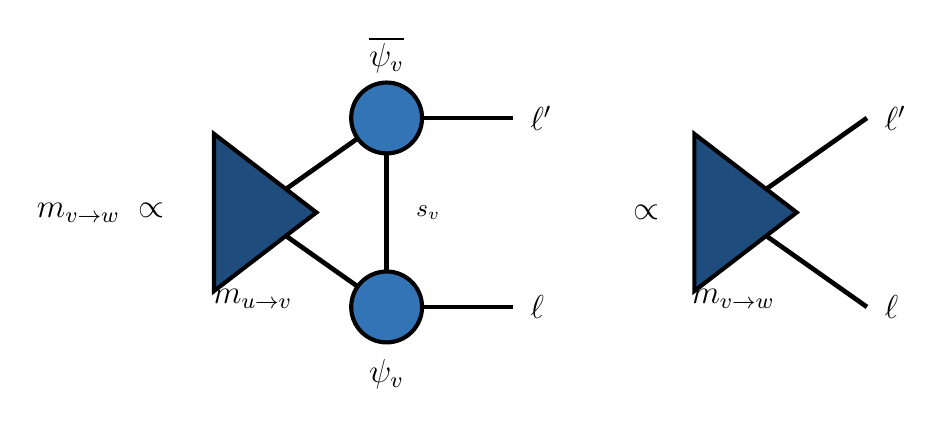
\begin{tikzpicture}
  \node[lab,anchor=east] at (-0.4,1.2) {$m_{v \to w} \;\propto$};
  % site v as its ket and bra, with the incoming matrix message from u and open bonds towards w
  \coordinate (M) at (0.6,1.2);
  \coordinate (k) at (2.3,0); \coordinate (b) at (2.3,2.4);
  \draw[leg] (M) -- (k); \draw[leg] (M) -- (b);
  \draw[leg] (k) -- (b);
  \draw[leg] (k) -- ++(1.6,0); \draw[leg] (b) -- ++(1.6,0);
  \node[msgmat] at (M) {};
  \node[tensor] at (k) {}; \node[tensor] at (b) {};
  \node[lab,anchor=north] at (0.6,0.35) {$m_{u \to v}$};
  \node[lab,anchor=west] at (2.55,1.2) {\small$s_v$};
  \node[lab] at (2.3,-0.85) {$\psi_v$};
  \node[lab] at (2.3,3.2) {$\overline{\psi_v}$};
  \node[lab,anchor=west] at (4.0,0.0) {$\ell$};
  \node[lab,anchor=west] at (4.0,2.4) {$\ell'$};
  % the result is again a matrix on the bond towards w
  \node[lab] at (5.6,1.2) {$\propto$};
  \coordinate (N) at (6.7,1.2);
  \draw[leg] (N) -- (8.4,0); \draw[leg] (N) -- (8.4,2.4);
  \node[msgmat] at (N) {};
  \node[lab,anchor=north] at (6.7,0.35) {$m_{v \to w}$};
  \node[lab,anchor=west] at (8.5,0.0) {$\ell$};
  \node[lab,anchor=west] at (8.5,2.4) {$\ell'$};
\end{tikzpicture}
\end{document}
